%! Author = Len Washington III
%! Date = 10/21/2023

% Preamble
\documentclass[19]{cs430lecture}
\usepackage{graphicx}

% Packages

% Document
\begin{document}

%<*Lecture-Activity-19>
\maketitle
\section{Fractional Knapsack Problem}\label{sec:fractional-knapsack-problem}
\answer{\begin{itemize}
	\item Prove optimal substructure
	\item Prove Greedy Choice
\end{itemize}}

\begin{enumerate}
    \item Prove that the Fractional Knapsack Problem has optimal substructure. \answer{\begin{itemize}
        \item What is the problem?
		\item Assume you have an optimal answer.
		\begin{equation*}
		\begin{aligned}
			p: &w_{1} , w_{2}, \dots, w_{n}\\
			   &v_{1}, v_{2}, \dots, v_{n}\\
			0 \leq f_{i} \leq &\mbox{ is the fractional amount of each item}\\
			&\sum_{subset\ 1\leq 1\leq n} f_{i}v_{i} \mbox{ is max}\\
			&\sum_{subset} f_{i}w_{i} \leq W
		\end{aligned}
		\end{equation*}
    \end{itemize}}
	\item Try various ``common sense'' greedy approaches that divide the problem into a sub-problem(s) and try to come up with counter-examples or prove the greedy choice is correct using the ``\hyperref[dfn:cut-and-paste]{cut and paste}'' proof.\answer{\begin{itemize}
		\item Max Value First -- if you fill the ``bag'' up immediately, you may miss out on a better value combination.\begin{table}[H]
		    \centering
		    \begin{threeparttable}
				\label{tab:max-first-counter}
				\begin{tabular}{c|c}
					$\mathbf{v_{i}}$ & $\mathbf{w_{i}}$\\
					\midrule
					10 & 5\\
					6 & 3\\
					5 & 2
				\end{tabular}
			\end{threeparttable}
		\end{table}
		\item Max $\left( \frac{v_{i}}{w_{i}} \right)$ first.
		In Greedy Order: $O(n\lg n)$ sort
		\begin{equation*}
		\begin{aligned}
			&\frac{v_{1}}{w_{1}} \geq \frac{v_{2}}{w_{2}} \geq \dots \geq \frac{v_{n}}{w_{n}}\\
			&\mbox{Assume fractional optimal answer } 0 \leq f \leq 1
		\end{aligned}
		\end{equation*}
		What is the optimal answer does not have the greedy choice?
		The optimal answer does not contain as much of item \#1 as possible.
		``\hyperref[dfn:cut-and-paste]{Cut and paste}'' proof
		Somet\_\_\_\_ greedy choice $w$ of item 1: $w_{1}$ of other items removed and the $value\ out \leq v_{1}$.
		The runtime is $O(n\lg n)$, sorting in $O(n\lg n)$ time and then just taking items.
	\end{itemize}}
\end{enumerate}

\section{Huffman Codes Problem}\label{sec:huffman-codes-problem}
Data Encoding Background
\begin{itemize}
	\item Data is a sequence of characters
	\item Fixed Length -- Each character is represented by a unique binary string.
	Easy to encode, concatenate the codes together. Easy to decode, break off 3-bit codewords and decode each one.
	\item Variable Length -- Give frequent characters shorter codewords, infrequent characters get long codewords.
	However, how do we decode if the length of the codewords are variable?
	\item Prefix Codes -- No codeword is a prefix of another codeword.
	Easy to encode, concatenate the code together.
	Easy to decode, since no codeword is a prefix of another, strip off one bit at a time and match to the unique prefix code
\end{itemize}


Huffman Codes
\begin{itemize}
	\item Are a Data Compression technique using a greedy algorithm to construct an optimal variable length prefix code
	\item Use frequency of occurrence of characters to build an optimal way to represent each character as a binary string
	\item Use a Binary tree method -- 0 means go to left child, 1 means go to right child (not a binary search tree).
	\item Cost of Tree in bits: \[ B(T) = \sum_{\mbox{for all } c\in C} \Call{freq}{c} \times \Call{\hyperref[sec:tree-depth-vs-tree-height]{depth}}{c} \]
\end{itemize}

Example
\begin{table}[H]
    \centering
    \begin{threeparttable}
		\caption{A character-coding problem. A data file of 100,000 characters containes only the characters a--f, with the frequencies indicated. If each character is assigned a 3-bit codeword, the file can be encoded in 300,000 bits. Using the variable-length code shown, the file can be encoded in 224,000 bits.}
		\label{tab:character-encoding-problem}
		\begin{tabular}{lcccccc}
						 & $a$ & $b$ & $c$ & $d$ & $e$ & $f$\\
			\midrule
			Frequency (in thousands)	& 45	& 13	& 12	& 16	& 9		& 5\\
			Fixed-length codeword		& 000	& 001	& 010	& 011	& 100	& 101\\
			Variable-length codeword	& 0		& 101	& 100	& 111	& 1101	& 1100
		\end{tabular}
		\begin{tablenotes}
			\small
			\item \answer{The 224,000 bit came from multiplying the freqency (in thousands) of each character by the length of the variable codeword, which would represent its height in the binary tree, as described in Figure~\ref{fig:19.1}.
			$45(1) + 13(3) + 12(3) + 16(3) + 9(4) + 5(4) = 45 + 39 + 36 + 48 + 36 + 20 = 224$.}
		\end{tablenotes}
	\end{threeparttable}
\end{table}

\begin{figure}[H]
	\centering
	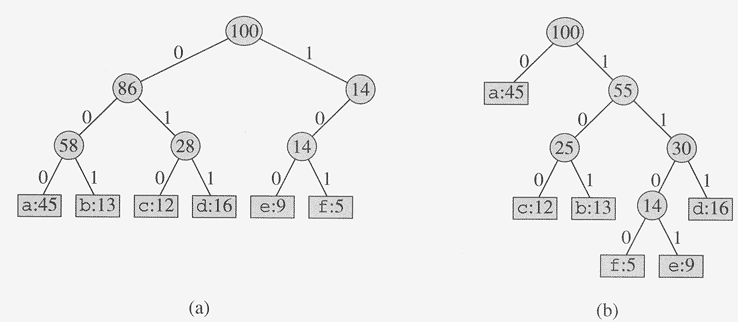
\includegraphics[width=\textwidth]{19.1}
	\caption{Trees corresponding to the coding schemes in Table~\ref{tab:character-encoding-problem}. Each leaf is labeled with a character and its frequency of occurence. Each internal node is labeled with the sum of the frequencies of the leaves in its subtree. \textbf{(a)} The tree corresponding to the fixed-length code $a=000, \dots, f=101$. \textbf{(b)} The tree corresponding to the optimal prefix code $a=0, b=101, \dots, f=1100$.}
	\label{fig:19.1}
\end{figure}
\begin{enumerate}[start=3]
    \item Prove that the Huffman Codes Problem has optimal substructure.\\
	\answer{Problem \begin{equation*}
	\begin{aligned}
		&c_{1}, c_{2}, \dots, c_{n} & \mbox{ characters}\\
		&f_{1}, f_{2}, \dots, f_{n} & \mbox{ frequency}\\
	\end{aligned}
	\end{equation*}
	Optimal Answer:\begin{equation*}
	\begin{aligned}
		&l_{1}, l_{2}, \dots, l_{n} \mbox{ bit length of variable length prefix code}\\
		&\sum_{i=1}^{n} f_{i}l_{i}\mbox{ is minimized}
	\end{aligned}
	\end{equation*}
	There is an encoder/decoder decision tree for this optimal answer.
	There must be a character in that optimal answer with the shortest (or one of the shortest if there are multiple) $l_{k}$.
	If you remove char $l_{k}$ from the problem, }
\end{enumerate}

The greedy approach is: Build the tree bottom up by using a minimum priority queue to merge 2 least frequent objects (objects are leaf nodes or other subtrees) together into a new subtree.

\begin{table}[H]
    \centering
    \begin{threeparttable}
		\label{tab:}
		\begin{tabular}{|c|c|}
			\toprule
			\begin{minipage}{0.5\textwidth}
				\begin{figure}[H]
					\centering
					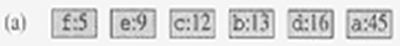
\includegraphics[width=\textwidth]{19.2}
					\label{fig:19.2}
				\end{figure}%
				\begin{figure}[H]
					\centering
					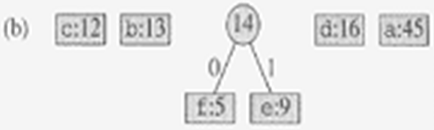
\includegraphics[width=\textwidth]{19.3}
					\label{fig:19.3}
				\end{figure}%
				\begin{figure}[H]
					\centering
					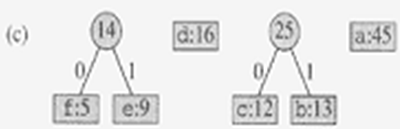
\includegraphics[width=\textwidth]{19.4}
					\label{fig:19.4}
				\end{figure}%
				\begin{figure}[H]
					\centering
					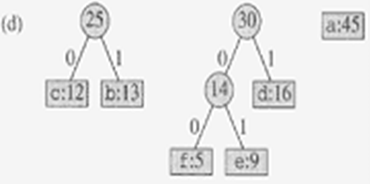
\includegraphics[width=\textwidth]{19.5}
					\label{fig:19.5}
				\end{figure}%
			\end{minipage} &
			\begin{minipage}{0.5\textwidth}
				\begin{figure}[H]
					\centering
					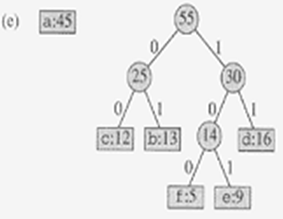
\includegraphics[width=\textwidth]{19.6}
					\label{fig:19.6}
				\end{figure}%
				\begin{figure}[H]
					\centering
					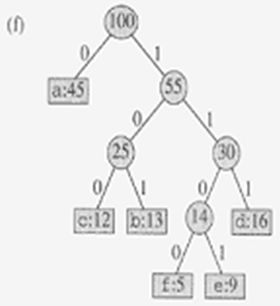
\includegraphics[width=\textwidth]{19.7}
					\label{fig:19.7}
				\end{figure}%
			\end{minipage}\\
			\bottomrule
		\end{tabular}
		\begin{tablenotes}
			\small
			\item Huffman \url{http://www.cs.auckland.ac.nz/software/AlgAnim/huffman.html}
		\end{tablenotes}
	\end{threeparttable}
\end{table}

\begin{enumerate}[start=4]
    \item Proof this greedy algorithm leads to an optimal Huffman Code tree: Build the tree bottom up by using a minimum priority queue to merge 2 least frequent objects (objects are leaf nodes or other subtrees) together into a new subtree.
\end{enumerate}

%</Lecture-Activity-19>

\end{document}